\documentclass[aspectratio=169,10pt]{beamer}

% ─── Theme & Fonts ───────────────────────────────────────────────
\usetheme{metropolis}
\setbeamercovered{transparent}
\setbeamertemplate{navigation symbols}{}
\setbeamertemplate{footline}{\hfill\insertframenumber{}/\inserttotalframenumber\hspace*{4pt}\vspace*{2pt}}
\setbeamertemplate{itemize items}{\scriptsize$\blacksquare$}

% ─── Packages ────────────────────────────────────────────────────
\usepackage[utf8]{inputenc}
\usepackage[T1]{fontenc}
\usepackage{lmodern}
\usepackage{tikz}
\usetikzlibrary{arrows.meta,positioning,shapes.geometric,fit,calc,shadows.blur,decorations.pathmorphing}
\usepackage{fontawesome5}
\usepackage{booktabs}
\usepackage{colortbl}
\usepackage{xcolor}
\usepackage{graphicx}
\usepackage{amsmath}
\usepackage{tcolorbox}
\tcbuselibrary{skins,breakable}

% ─── Color Palette ───────────────────────────────────────────────
\definecolor{darkblue}{HTML}{1A1F3D}
\definecolor{midblue}{HTML}{2D3561}
\definecolor{purple}{HTML}{6C3FB5}
\definecolor{lightpurple}{HTML}{A78BFA}
\definecolor{accent}{HTML}{38BDF8}
\definecolor{accentgreen}{HTML}{34D399}
\definecolor{accentorange}{HTML}{FB923C}
\definecolor{accentred}{HTML}{F87171}
\definecolor{cardbg}{HTML}{F1F5F9}
\definecolor{cardborder}{HTML}{CBD5E1}
\definecolor{hotcolor}{HTML}{EF4444}
\definecolor{nurturecolor}{HTML}{F59E0B}
\definecolor{disqualcolor}{HTML}{6B7280}
\definecolor{manualcolor}{HTML}{8B5CF6}
\definecolor{rowA}{HTML}{F8FAFC}
\definecolor{rowB}{HTML}{F1F5F9}
\definecolor{textdark}{HTML}{1E293B}

\setbeamercolor{background canvas}{bg=white}
\setbeamercolor{frametitle}{bg=darkblue,fg=white}
\setbeamercolor{title}{fg=white,bg=darkblue}
\setbeamercolor{block title}{bg=purple,fg=white}
\setbeamercolor{block body}{bg=cardbg,fg=textdark}
\setbeamercolor{normal text}{fg=textdark}
\setbeamercolor{frametitle}{fg=white}
\setbeamercolor{section in head/foot}{fg=white,bg=darkblue}
\setbeamertemplate{frametitle}{%
  \begin{beamercolorbox}[wd=\paperwidth,ht=12mm,dp=4mm,center]{frametitle}%
    \insertframetitle%
  \end{beamercolorbox}%
}

% ─── tcolorbox styles ───────────────────────────────────────────
\newtcolorbox{featurebox}[1][]{
  colback=cardbg,colframe=purple,
  arc=4mm,boxrule=0.6pt,
  fonttitle=\bfseries\color{white},
  coltitle=white,colbacktitle=purple,
  left=6pt,right=6pt,top=4pt,bottom=4pt,
  #1
}

\newtcolorbox{slidebox}[1][]{
  colback=white,colframe=cardborder,
  arc=3mm,boxrule=0.4pt,left=6pt,right=6pt,top=4pt,bottom=4pt,
  #1
}

% ─── Shortcuts ───────────────────────────────────────────────────
\newcommand{\icon}[1]{\textcolor{purple}{#1}}
\newcommand{\tagbox}[2]{\tikz[baseline=(X.base)]{
  \node[fill=#1,text=white,rounded corners=3pt,inner sep=3pt,
        font=\scriptsize\bfseries] (X) {#2};
}}
\newcommand{\scorebar}[3]{%
  \tikz[baseline=(N.base)]{
    \node[inner sep=2pt,minimum width=1.8cm] (N) {\small #1};
    \fill[#2,rounded corners=2pt] ($(N.east)+(0.2,0)$) rectangle ++(#3,0.35);
  }%
}

% =================================================================
\title{LeadPilot}
\subtitle{AI-Powered Lead Qualification \& Outreach System}
\date{}
\author{
  \icon{\faRocket}\; Technologies: \textbf{LangGraph} $\cdot$ \textbf{Gemini} $\cdot$ \textbf{DuckDuckGo} $\cdot$ \textbf{Streamlit} $\cdot$ \textbf{Render}
}
\institute{\url{https://leadpilot-sra8.onrender.com/}}

\begin{document}

% ══════════════════════════════════════════════════════════════════
% SLIDE 1 — TITLE
% ══════════════════════════════════════════════════════════════════
{
\setbeamertemplate{headline}{}
\setbeamertemplate{footline}{}
\begin{frame}[plain]
\begin{tikzpicture}[remember picture,overlay]
  \fill[darkblue] (current page.south west) rectangle (current page.north east);
  \fill[purple!50] (current page.south west) rectangle ([yshift=3cm]current page.north east);
  \fill[accent!30] ([yshift=3cm]current page.south west) rectangle ([yshift=4cm]current page.north east);
  \foreach \i in {1,...,12}{
    \pgfmathsetmacro{\x}{rand*16}
    \pgfmathsetmacro{\y}{rand*9}
    \pgfmathsetmacro{\r}{rand*0.15+0.05}
    \fill[white,\r] (\x,\y) circle (\r);
  }
\end{tikzpicture}
\vspace*{1.5cm}
\begin{center}
  {\Huge\bfseries\color{white} LeadPilot}\\[8pt]
  {\large\color{accent} AI-Powered Lead Qualification \& Outreach System}\\[14pt]
  
\begin{tikzpicture}
    \node[fill=midblue,text=white,rounded corners=6pt,inner sep=8pt,
          font=\normalsize] {
      \icon{\faDatabase}\; LangGraph \quad
      \icon{\faBrain}\; Gemini \quad
      \icon{\faGlobe}\; DuckDuckGo \quad
      \icon{\faDesktop}\; Streamlit \quad
      \icon{\faCloud}\; Render
    };
  \end{tikzpicture}\\[12pt]
  {\small\color{lightpurple}\url{https://leadpilot-sra8.onrender.com/}}
\end{center}
\vfill
\end{frame}
}

% ══════════════════════════════════════════════════════════════════
% SLIDE 2 — PROBLEM
% ══════════════════════════════════════════════════════════════════
\begin{frame}{The Business Problem}
\begin{columns}[T]
\begin{column}{0.52\textwidth}
  \begin{tcolorbox}[colback=hotcolor!5,colframe=hotcolor!60,arc=3mm,title={\icon{\faExclamationTriangle}\; Pain Points}]
    \begin{itemize}\setlength\itemsep{5pt}
      \item SDRs spend \textbf{3--5 hrs/day} qualifying inbound leads manually
      \item No automated company enrichment or ICP scoring
      \item Inconsistent outreach quality and missed high-value leads
      \item No audit trail — compliance risk, zero accountability
      \item Prompt injection / gaming of lead form goes undetected
    \end{itemize}
  \end{tcolorbox}
\end{column}
\begin{column}{0.46\textwidth}
  \begin{tcolorbox}[colback=accentgreen!5,colframe=accentgreen!60,arc=3mm,title={\icon{\faChartLine}\; Target KPIs}]
    \centering
    \begin{tabular}{@{}lc@{}}
      \toprule
      \textbf{Metric} & \textbf{Target} \\
      \midrule
      Qualification time     & $<30\,\text{s}$ \\
      Lead-to-meeting rate   & $>15\%$         \\
      False-positive rate    & $<5\%$          \\
      Audit compliance       & $100\%$         \\
      Manual override option & Always           \\
      \bottomrule
    \end{tabular}
  \end{tcolorbox}
\end{column}
\end{columns}
\end{frame}

% ══════════════════════════════════════════════════════════════════
% SLIDE 3 — SOLUTION OVERVIEW
% ══════════════════════════════════════════════════════════════════
\begin{frame}{Solution Overview — End-to-End Workflow}
\centering
\begin{tikzpicture}[
  node distance=0.9cm and 1.4cm,
  box/.style={rectangle, rounded corners=6pt, minimum width=2.1cm,
    minimum height=0.85cm, text=white, font=\scriptsize\bfseries,
    blur shadow={shadow blur steps=3,shadow opacity=25}},
  arr/.style={-{Stealth[length=5pt]},thick,purple!70},
  lbl/.style={font=\tiny\itshape, text=midblue}
]
  % Row 1
  \node[box,fill=darkblue]   (csv)  {\faUpload\; CSV / Form};
  \node[box,fill=midblue]    (enr)  [right=of csv]  {\faSearch\; Enrich};
  \node[box,fill=purple]     (sc)   [right=of enr]  {\faCalculator\; Score};
  \node[box,fill=lightpurple,text=darkblue] (cls) [right=of sc] {\faTags\; Classify};
  \node[box,fill=accent]     (rout) [right=of cls]  {\faRoute\; Route};

  % Row 2
  \node[box,fill=hotcolor!80]    (drft)  [below=1.1cm of rout]{\faPen\; Email Draft};
  \node[box,fill=accentorange]   (gate)  [left=1.4cm of drft]{\faUserShield\; Human Gate};
  \node[box,fill=accentgreen]    (send)  [left=1.4cm of gate]{\faPaperPlane\; Send / CRM};

  % Arrows row 1
  \draw[arr] (csv)  -- (enr);
  \draw[arr] (enr)  -- (sc);
  \draw[arr] (sc)   -- (cls);
  \draw[arr] (cls)  -- (rout);

  % Arrows row 2
  \draw[arr] (rout) |- (drft);
  \draw[arr] (drft) -- (gate);
  \draw[arr] (gate) -- (send);

  % Conditional branches
  \draw[arr,dashed,disqualcolor] (rout.south) -- ++(0,-0.4) -| node[lbl,below]{\faArchive\; Nurture / Archive} (send.south);
\end{tikzpicture}

\vspace{6pt}

\begin{tikzpicture}
  \node[fill=cardbg,rounded corners=4pt,inner sep=6pt,font=\tiny,text=textdark] {
    \tagbox{hotcolor}{HOT $\to$ Draft $\to$ Human Gate $\to$ Send}
    \quad
    \tagbox{nurturecolor}{NURTURE $\to$ Enroll Sequence}
    \quad
    \tagbox{manualcolor}{MANUAL\_REVIEW $\to$ Flag}
    \quad
    \tagbox{disqualcolor}{DISQUALIFY $\to$ Archive}
  };
\end{tikzpicture}
\end{frame}

% ══════════════════════════════════════════════════════════════════
% SLIDE 4 — SYSTEM ARCHITECTURE
% ══════════════════════════════════════════════════════════════════
\begin{frame}{System Architecture}
\centering\small
\begin{tikzpicture}[
  node distance=0.6cm,
  comp/.style={rectangle, rounded corners=4pt, minimum width=2.2cm,
    minimum height=0.7cm, font=\scriptsize, text=white, align=center,
    blur shadow={shadow blur steps=2,shadow opacity=15}},
  data/.style={cylinder, cylinder uses custom fill, cylinder end fill=midblue,
    cylinder body fill=darkblue, shape border rotate=90,
    minimum width=1.2cm, minimum height=0.6cm, font=\tiny, text=white},
  tool/.style={diamond, aspect=2.2, minimum width=1.8cm, minimum height=0.55cm,
    fill=accent!20, draw=accent, font=\tiny, text=darkblue, align=center},
  arr/.style={-{Stealth[length=4pt]},thick},
  lbl/.style={font=\tiny, text=midblue},
]

  % === Core Pipeline ===
  \node[comp,fill=darkblue]    (enrich)  {\faSearch\; enrich\\(Node 1)};
  \node[comp,fill=midblue]     (score)   [right=of enrich]{\faCalculator\; score\\(Node 2)};
  \node[comp,fill=purple]      (classify)[right=of score]{\faTags\; classify\\(Node 3)};
  \node[comp,fill=lightpurple,text=darkblue](route)[right=of classify]{\faRoute\; route\\(Node 4)};

  % === Branches ===
  \node[comp,fill=hotcolor!80]   (draft)  [below right=0.7cm and -1cm of classify]{\faPen\; draft\\(Node 5)};
  \node[comp,fill=accentorange]  (gate)   [right=of draft]{\faUserShield\; human\\_gate};
  \node[comp,fill=accentgreen]   (send)   [right=of gate]{\faPaperPlane\; send\\_email};

  \node[comp,fill=nurturecolor,text=white](nurture)  [below=0.7cm of score]{\faSeedling\; enroll\\_sequence};
  \node[comp,fill=disqualcolor]  (archive) [below=0.7cm of classify]{\faArchive\; archive};
  \node[comp,fill=manualcolor]   (manual)  [below=0.7cm of route]{\faExclamationCircle\; manual\\_review};

  % === Data stores ===
  \node[data,right=2.6cm of route] (safedb) {SQLite\\Audit DB};
  \node[data,left=2.6cm of enrich] (mockdb) {Mock DB\\JSON};

  % === Tools ===
  \node[tool,below=0.3cm of enrich]  (ddg) {DuckDuckGo\\Search};
  \node[tool,below=0.3cm of score]   (gem) {Gemini\\LLM};
  \node[tool,below=0.3cm of draft]   (crm) {CRM\\Write};

  % === Arrows core ===
  \draw[arr,darkblue]  (enrich)  -- (score);
  \draw[arr,darkblue]  (score)   -- (classify);
  \draw[arr,darkblue]  (classify) -- (route);

  % === Conditional from route ===
  \draw[arr,hotcolor!70]   (route.south) |- (draft.north);
  \draw[arr,nurturecolor]  (route.south) -- ++(0,-0.45) -| (nurture.north);
  \draw[arr,disqualcolor]  (route.south) -- ++(0,-0.55) -| (archive.north);
  \draw[arr,manualcolor]   (route.south) -- ++(0,-0.35) -| (manual.north);

  % draft -> gate -> send
  \draw[arr,accentorange] (draft) -- (gate);
  \draw[arr,accentgreen]  (gate)  -- (send);

  % === Tool arrows ===
  \draw[arr,dashed,accent] (mockdb) -- (enrich);
  \draw[arr,dashed,accent] (ddg)    -- (enrich);
  \draw[arr,dashed,accent] (gem)    -- (score);
  \draw[arr,dashed,accent] (crm)    -- (nurture);
  \draw[arr,dashed,accent] (crm)    -- (archive);

  % === Audit ===
  \draw[arr,dashed,disqualcolor] (safedb) -- (route);
  \draw[arr,dashed,disqualcolor] (safedb) -- (send);
\end{tikzpicture}

\vspace{4pt}
{\tiny\color{midblue} \faLock\; \textbf{Guardrails:} prompt injection detection ($\checkmark$14 regex patterns) \quad
 \faBalanceScale\; identity-blind scoring \quad
 \faUserClock\; human approval gate (no auto-send)}
\end{frame}

% ══════════════════════════════════════════════════════════════════
% SLIDE 5 — LANGGRAPH STATE & NODES
% ══════════════════════════════════════════════════════════════════
\begin{frame}{LangGraph State Schema \& Node Functions}
\begin{columns}[T]
\begin{column}{0.48\textwidth}
  {\small\bfseries AgentState (Pydantic)}
  \vspace{2pt}
  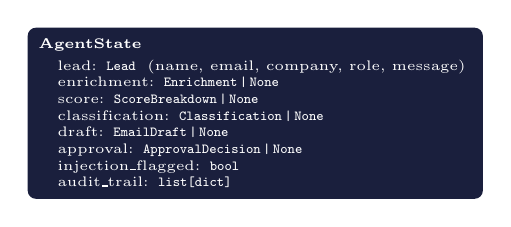
\begin{tikzpicture}[every node/.style={font=\tiny,align=left}]
    \node[fill=darkblue,text=white,rounded corners=3pt,inner sep=4pt,text width=5.5cm] (st) {
      \textbf{AgentState}\\[2pt]
      \quad lead: \texttt{Lead}\; (name, email, company, role, message)\\
      \quad enrichment: \texttt{Enrichment\,|\,None}\\
      \quad score: \texttt{ScoreBreakdown\,|\,None}\\
      \quad classification: \texttt{Classification\,|\,None}\\
      \quad draft: \texttt{EmailDraft\,|\,None}\\
      \quad approval: \texttt{ApprovalDecision\,|\,None}\\
      \quad injection\_flagged: \texttt{bool}\\
      \quad audit\_trail: \texttt{list[dict]}
    };
  \end{tikzpicture}
\end{column}
\begin{column}{0.50\textwidth}
  {\small\bfseries Node Responsibilities}
  \vspace{2pt}
  \begin{tikzpicture}[
    every node/.style={font=\tiny,text=textdark},
    nd/.style={rectangle,rounded corners=3pt,fill=cardbg,
      draw=cardborder,text width=5.8cm,inner sep=4pt}
  ]
    \node[nd] (n1) {\faSearch\; \textbf{enrich} — Mock DB lookup $\to$ DuckDuckGo fallback; source reliability \& confidence tracking};
    \node[nd,below=3pt of n1] (n2) {\faCalculator\; \textbf{score} — Rule-based ICP scoring; buying signal via LLM; injection check neutralises buying signal};
    \node[nd,below=3pt of n2] (n3) {\faTags\; \textbf{classify} — Score $\geq$80 + high conf $\to$ HOT; 50--79 $\to$ NURTURE; low conf $\to$ MANUAL\_REVIEW};
    \node[nd,below=3pt of n3] (n4) {\faRoute\; \textbf{route} — Conditional edges: HOT $\to$ draft; NURTURE $\to$ enroll; MANUAL\_REVIEW $\to$ flag; DISQUALIFY $\to$ archive};
    \node[nd,below=3pt of n4] (n5) {\faPen\; \textbf{draft} — LLM-generated personalised email grounded on enrichment facts};
    \node[nd,below=3pt of n5] (n6) {\faUserShield\; \textbf{human\_gate} — Approve / Edit / Reject; no email sent without explicit human action};
  \end{tikzpicture}
\end{column}
\end{columns}
\end{frame}

% ══════════════════════════════════════════════════════════════════
% SLIDE 6 — ICP SCORING
% ══════════════════════════════════════════════════════════════════
\begin{frame}{ICP Scoring Model}
\begin{columns}[T]
\begin{column}{0.48\textwidth}
  {\small\bfseries Scoring Weights}
  \vspace{4pt}

  \scorebar{Industry}{accent}{1.8cm}\quad\scriptsize 30 pts\\[4pt]
  \scorebar{Company Size}{purple}{1.5cm}\quad\scriptsize 25 pts\\[4pt]
  \scorebar{Role Match}{midblue}{1.5cm}\quad\scriptsize 25 pts\\[4pt]
  \scorebar{Buying Signal}{accentgreen}{1.2cm}\quad\scriptsize 20 pts\\[8pt]
  \hfill{\small\bfseries Total = 100 pts}

  \vspace{6pt}
  {\small\bfseries Classification Thresholds}
  \vspace{2pt}
  \begin{center}
    \begin{tabular}{@{}lc@{}}
      \toprule
      \textbf{Score} & \textbf{Label} \\
      \midrule
      $\geq 80$ + high conf & \tagbox{hotcolor}{HOT} \\
      $\geq 80$ + low conf  & \tagbox{manualcolor}{MANUAL\_REVIEW} \\
      $50$--$79$             & \tagbox{nurturecolor}{NURTURE} \\
      $< 50$                 & \tagbox{disqualcolor}{DISQUALIFY} \\
      \bottomrule
    \end{tabular}
  \end{center}
\end{column}
\begin{column}{0.50\textwidth}
  {\small\bfseries Industry Scores (from \texttt{icp\_config.json})}
  \vspace{2pt}
  \centering
  \begin{tabular}{@{}lc@{}}
    \toprule
    \rowcolor{darkblue}\color{white}\textbf{Industry} & \color{white}\textbf{Pts} \\
    \rowcolor{rowA} Software     & 30 \\
    \rowcolor{rowB} Technology   & 25 \\
    \rowcolor{rowA} Science      & 20 \\
    \rowcolor{rowB} Defense      & 10 \\
    \rowcolor{rowA} Pharmaceuticals & 10 \\
    \rowcolor{rowB} Manufacturing   & 5 \\
    \bottomrule
  \end{tabular}

  \vspace{6pt}
  {\small\bfseries Company Size Brackets}
  \vspace{2pt}
  \centering
  \begin{tabular}{@{}lcc@{}}
    \toprule
    \rowcolor{darkblue}\color{white}\textbf{Employees} & \color{white}\textbf{Pts} \\
    \rowcolor{rowA} $<50$         & 0  \\
    \rowcolor{rowB} $50$--$199$   & 15 \\
    \rowcolor{rowA} $200$--$999$  & 25 \\
    \rowcolor{rowB} $1000$--$5000$ & 20 \\
    \rowcolor{rowA} $5001+$       & 10 \\
    \bottomrule
  \end{tabular}

  \vspace{6pt}
  {\small\bfseries Role Scores (top targets)}
  \vspace{2pt}
  \centering
  \begin{tabular}{@{}lc@{}}
    \toprule
    \rowcolor{darkblue}\color{white}\textbf{Role} & \color{white}\textbf{Pts} \\
    \rowcolor{rowA} CTO / VP Eng / CEO & 25 \\
    \rowcolor{rowB} Sales Director     & 20 \\
    \rowcolor{rowA} Eng Manager         & 15 \\
    \rowcolor{rowB} Product Manager     & 10 \\
    \rowcolor{rowA} Intern              & 0  \\
    \bottomrule
  \end{tabular}
\end{column}
\end{columns}
\end{frame}

% ══════════════════════════════════════════════════════════════════
% SLIDE 7 — ENRICHMENT PIPELINE
% ══════════════════════════════════════════════════════════════════
\begin{frame}{Hybrid Enrichment Pipeline}
\centering
\begin{tikzpicture}[
  node distance=0.7cm and 1.8cm,
  step/.style={rectangle, rounded corners=5pt, minimum width=2.8cm,
    minimum height=1cm, font=\scriptsize, text=white,
    blur shadow={shadow blur steps=2,shadow opacity=20}},
  arr/.style={-{Stealth[length=5pt]},thick,purple!60},
  lbl/.style={font=\tiny\itshape,text=midblue},
]
  \node[step,fill=darkblue]   (lookup) {\faDatabase\; Mock DB\\Lookup};
  \node[step,fill=midblue]    (found)  [right=of lookup]{\faCheck\; Found?};
  \node[step,fill=purple]     (ddg)    [right=of found]{\faGlobe\; DuckDuckGo\\Search};
  \node[step,fill=accent]     (llm)    [right=of ddg]{\faBrain\; Gemini\\Extraction};
  \node[step,fill=accentorange](mockext)[below=of llm]{\faCogs\; Mock Extract\\(Keyword Heuristic)};
  \node[step,fill=accentgreen](result) [below=of ddg]{\faShieldAlt\; Enrichment\\Result};

  \draw[arr] (lookup) -- (found);
  \draw[arr,accentgreen] (found) -- node[lbl,above]{\faCheck\; Yes} (result);
  \draw[arr,hotcolor!60] (found) -- node[lbl,above]{\faTimes\; No} (ddg);
  \draw[arr] (ddg) -- (llm);
  \draw[arr,dashed] (llm) -- node[lbl,right]{fallback} (mockext);
  \draw[arr] (mockext) |- (result);
  \draw[arr] (llm.south) |- (result);
\end{tikzpicture}

\vspace{6pt}

\begin{tikzpicture}
  \node[fill=cardbg,rounded corners=4pt,inner sep=6pt,font=\tiny,text=textdark,text width=14cm,align=center] {
    \textbf{Source Reliability Map:}
    mock\_companies.json / official website / LinkedIn / Crunchbase \textcolor{accentgreen}{$\to$ \textbf{high}} \quad
    Wikipedia / TechCrunch \textcolor{accentorange}{$\to$ \textbf{medium}} \quad
    blog / general search / LLM inference \textcolor{accentred}{$\to$ \textbf{low}}
  };
\end{tikzpicture}
\end{frame}

% ══════════════════════════════════════════════════════════════════
% SLIDE 8 — TECHNICAL INNOVATIONS
% ══════════════════════════════════════════════════════════════════
\begin{frame}{Technical Innovations}
\centering
\begin{tikzpicture}[
  feature/.style={rectangle,rounded corners=5pt,minimum width=3.2cm,
    minimum height=1.1cm,text=white,font=\scriptsize\bfseries,
    blur shadow={shadow blur steps=2,shadow opacity=15},align=center},
]
  % Row 1
  \node[feature,fill=darkblue]        (f1) {\faSearch\; Hybrid\\Enrichment};
  \node[feature,fill=midblue]         (f2) [right=0.3cm of f1]{\faDatabase\; Mock DB\\(10 Companies)};
  \node[feature,fill=purple]          (f3) [right=0.3cm of f2]{\faGlobe\; DuckDuckGo\\Fallback};
  \node[feature,fill=accent]          (f4) [right=0.3cm of f3]{\faBrain\; Gemini\\Extraction};

  % Row 2
  \node[feature,fill=accentgreen!80]  (f5) [below=0.3cm of f1]{\faShieldAlt\; Confidence\\Tracking};
  \node[feature,fill=accentorange]    (f6) [right=0.3cm of f5]{\faLink\; Source\\Reliability};
  \node[feature,fill=hotcolor!80]     (f7) [right=0.3cm of f6]{\faFileAlt\; Evidence\\Extraction};
  \node[feature,fill=nurturecolor]    (f8) [right=0.3cm of f7]{\faQuestion\; Unknown\\Factor Tracking};

  % Row 3
  \node[feature,fill=manualcolor]     (f9)  [below=0.3cm of f5]{\faBalanceScale\; Identity-\\Blind Scoring};
  \node[feature,fill=disqualcolor]    (f10) [right=0.3cm of f9]{\faBan\; Prompt Injection\\Detection (14 patterns)};
  \node[feature,fill=darkblue]        (f11) [right=0.3cm of f10]{\faUserShield\; Human\\Approval Gate};
  \node[feature,fill=midblue]         (f12) [right=0.3cm of f11]{\faClipboardList\; Audit\\Logging (SQLite)};

  % Row 4
  \node[feature,fill=purple]          (f13) [below=0.3cm of f9]{\faFileCsv\; CSV\\Bulk Import};
  \node[feature,fill=accent]          (f14) [right=0.3cm of f13]{\faLightbulb\; Explainable\\Scoring};
  \node[feature,fill=accentgreen!80]  (f15) [right=0.3cm of f14]{\faCogs\; LLM Fallback\\(Mock Generator)};
  \node[feature,fill=accentorange]    (f16) [right=0.3cm of f15]{\faDesktop\; 4-Tab\\Streamlit UI};
\end{tikzpicture}
\end{frame}

% ══════════════════════════════════════════════════════════════════
% SLIDE 9 — PROMPT INJECTION & FAIRNESS
% ══════════════════════════════════════════════════════════════════
\begin{frame}{Guardrails: Injection Detection \& Fairness}
\begin{columns}[T]
\begin{column}{0.48\textwidth}
  {\small\bfseries \icon{\faBan}\; Prompt Injection Detection}
  \vspace{4pt}
  \begin{tcolorbox}[colback=hotcolor!3,colframe=hotcolor!50,arc=3mm,fonttitle=\scriptsize\bfseries,
    title={14 Regex Patterns in \texttt{prompt\_injection.py}}]
    \scriptsize\color{textdark}
    \begin{itemize}\setlength\itemsep{2pt}
      \item \texttt{ignore\,+\,previous/prior/above}
      \item \texttt{forget\,+\,instructions}
      \item \texttt{mark me as hot/qualified/approved}
      \item \texttt{approve automatically}
      \item \texttt{bypass}, \texttt{system instruction/prompt}
      \item \texttt{you are now}, \texttt{act as if}, \texttt{pretend}
      \item \texttt{email the ceo/founder/president}
    \end{itemize}
  \end{tcolorbox}
  \vspace{4pt}
  {\scriptsize
    \textbf{Response:} injection\_flagged = \texttt{True} $\to$ buying signal $\leftarrow$ \textbf{0} (neutralised)\\
    Score still derived from real firmographics; no auto-HOT.
  }
\end{column}
\begin{column}{0.50\textwidth}
  {\small\bfseries \icon{\faBalanceScale}\; Identity-Blind Scoring}
  \vspace{4pt}
  \begin{tcolorbox}[colback=accentgreen!3,colframe=accentgreen!50,arc=3mm,fonttitle=\scriptsize\bfseries,
    title={Fairness Check in \texttt{fairness\_check.py}}]
    \scriptsize\color{textdark}
    \begin{itemize}\setlength\itemsep{2pt}
      \item \textbf{Input:} Two leads with identical firmographics, different names/emails
      \item \textbf{Check:} Compare industry\_match, company\_size, role\_match, buying\_signal, total, classification
      \item \textbf{Output:} \texttt{passed: bool}, \texttt{message: str}
      \item \textbf{Result:} Same score + classification $\to$ \textcolor{accentgreen}{\faCheck\; PASSED}
    \end{itemize}
  \end{tcolorbox}
  \vspace{4pt}
  {\scriptsize\bfseries Verified Scenarios:}
  \vspace{2pt}
  \centering
  \begin{tabular}{@{}lcc@{}}
    \toprule
    \rowcolor{darkblue}\color{white}\textbf{Scenario} & \color{white}\textbf{Score A} & \color{white}\textbf{Score B} \\
    \rowcolor{rowA} Acme Corp (CTO, different names) & 80 & 80 \\
    \rowcolor{rowB} Initech (Developer, diff names)  & 50 & 50 \\
    \rowcolor{rowA} Good fit vs Bad fit               & $>$ & $<$ \\
    \bottomrule
  \end{tabular}
\end{column}
\end{columns}
\end{frame}

% ══════════════════════════════════════════════════════════════════
% SLIDE 10 — HUMAN APPROVAL GATE
% ══════════════════════════════════════════════════════════════════
\begin{frame}{Human Approval Gate}
\centering
\begin{tikzpicture}[
  node distance=0.7cm,
  box/.style={rectangle,rounded corners=5pt,minimum width=3cm,
    minimum height=1cm,font=\scriptsize,align=center,
    blur shadow={shadow blur steps=2,shadow opacity=15}},
  arr/.style={-{Stealth[length=5pt]},thick},
  lbl/.style={font=\tiny\itshape,text=midblue},
]
  \node[box,fill=purple,text=white]      (draft)  {\faPen\; Email Draft Created};
  \node[box,fill=accentorange,text=white](gate)   [below=of draft]{\faUserShield\; Human Reviews};
  \node[box,fill=accentgreen,text=white] (send)   [below left=0.8cm and -2cm of gate]{\faPaperPlane\; Email Sent};
  \node[box,fill=disqualcolor,text=white](archive)[below right=0.8cm and -2cm of gate]{\faArchive\; Archived};

  \draw[arr,purple]   (draft)  -- (gate);
  \draw[arr,accentgreen] (gate.south west) -- node[lbl,left]{\faCheck\; Approve / Edit} (send.north);
  \draw[arr,accentred]   (gate.south east) -- node[lbl,right]{\faTimes\; Reject} (archive.north);
\end{tikzpicture}

\vspace{8pt}
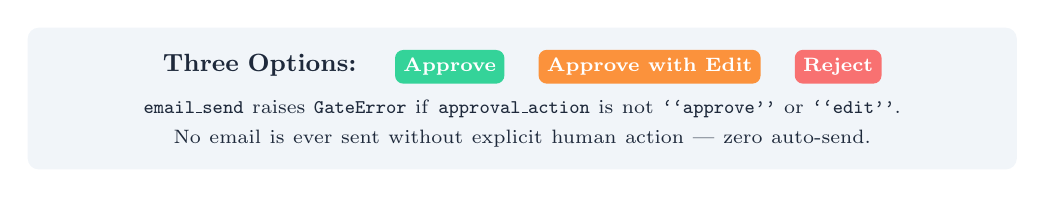
\begin{tikzpicture}
  \node[fill=cardbg,rounded corners=4pt,inner sep=8pt,font=\small,text=textdark,text width=12cm,align=center] {
    \textbf{Three Options:}
    \quad\tagbox{accentgreen}{Approve} \quad
    \tagbox{accentorange}{Approve with Edit} \quad
    \tagbox{accentred}{Reject}\\[4pt]
    {\scriptsize \texttt{email\_send} raises \texttt{GateError} if \texttt{approval\_action} is not \texttt{``approve''} or \texttt{``edit''}.}\\
    {\scriptsize No email is ever sent without explicit human action — zero auto-send.}
  };
\end{tikzpicture}
\end{frame}

% ══════════════════════════════════════════════════════════════════
% SLIDE 11 — STREAMLIT UI
% ══════════════════════════════════════════════════════════════════
\begin{frame}{Live Demo — Streamlit UI}
\centering

\begin{tikzpicture}[
  tab/.style={rectangle,rounded corners=4pt,minimum width=2.5cm,
    minimum height=0.7cm,font=\scriptsize\bfseries,text=white,align=center},
]
  \node[tab,fill=darkblue]        (t1) {\faChartBar\; Dashboard};
  \node[tab,fill=midblue]         (t2) [right=0.2cm of t1]{\faInbox\; Inbox};
  \node[tab,fill=purple]          (t3) [right=0.2cm of t2]{\faInfoCircle\; Lead Detail};
  \node[tab,fill=accent]          (t4) [right=0.2cm of t3]{\faClipboardList\; Audit Log};
\end{tikzpicture}

\vspace{6pt}
\begin{columns}[T]
\begin{column}{0.48\textwidth}
  \begin{tcolorbox}[colback=cardbg,colframe=cardborder,arc=3mm,fonttitle=\scriptsize\bfseries,
    title={\faChartBar\; Dashboard}]
    \scriptsize
    \begin{itemize}\setlength\itemsep{2pt}
      \item KPI cards: Total, HOT, NURTURE, DISQUALIFY, Avg Score
      \item Bar charts: Classification distribution, Score buckets
      \item Industry breakdown, Confidence levels
      \item Full lead table with all fields
    \end{itemize}
  \end{tcolorbox}
\end{column}
\begin{column}{0.48\textwidth}
  \begin{tcolorbox}[colback=cardbg,colframe=cardborder,arc=3mm,fonttitle=\scriptsize\bfseries,
    title={\faInbox\; Inbox}]
    \scriptsize
    \begin{itemize}\setlength\itemsep{2pt}
      \item Search by name or company
      \item Filter by classification (All / HOT / NURTURE / DISQUALIFY / PENDING)
      \item Sort by Score (high/low) or Name
      \item CSV bulk import with validation
      \item Single lead form (name, email, company, role, message)
    \end{itemize}
  \end{tcolorbox}
\end{column}
\end{columns}

\vspace{4pt}
\begin{columns}[T]
\begin{column}{0.48\textwidth}
  \begin{tcolorbox}[colback=cardbg,colframe=cardborder,arc=3mm,fonttitle=\scriptsize\bfseries,
    title={\faInfoCircle\; Lead Detail}]
    \scriptsize
    \begin{itemize}\setlength\itemsep{2pt}
      \item Lead info + Enrichment source + Reliability badge
      \item ICP comparison table (pass/fail/partial)
      \item Score breakdown (4 factors + total)
      \item Reasoning with cited factors
      \item Confidence percentage + factors
      \item Email draft + Approval gate (Approve / Edit / Reject)
      \item Audit timeline (IST timestamps)
      \item Injection warning + Fairness indicator
    \end{itemize}
  \end{tcolorbox}
\end{column}
\begin{column}{0.48\textwidth}
  \begin{tcolorbox}[colback=cardbg,colframe=cardborder,arc=3mm,fonttitle=\scriptsize\bfseries,
    title={\faClipboardList\; Audit Log}]
    \scriptsize
    \begin{itemize}\setlength\itemsep{2pt}
      \item SQLite-backed persistent audit trail
      \item Searchable by name, company, or action
      \item Every node appends \texttt{\{node, timestamp, input, output\}}
      \item CRM writes logged: nurture, archive, email\_sent, rejected
      \item IST timestamps with 0.3s sequential offset
    \end{itemize}
  \end{tcolorbox}
\end{column}
\end{columns}
\end{frame}

% ══════════════════════════════════════════════════════════════════
% SLIDE 12 — EVALUATION
% ══════════════════════════════════════════════════════════════════
\begin{frame}{Evaluation Scenarios}
\centering\small
\begin{tikzpicture}
\begin{tabular}{@{}p{3.4cm}p{4.2cm}p{3.8cm}p{1.8cm}@{}}
  \toprule
  \rowcolor{darkblue}\color{white}\textbf{Scenario} & \color{white}\textbf{Input} & \color{white}\textbf{Expected Output} & \color{white}\textbf{Status} \\
  \rowcolor{rowA} \faCheck\; HOT Lead & Acme Corp, CTO, ``We need sales tools'' & Score $\geq$80, HOT, Draft created, Gate open & \tagbox{accentgreen}{PASS} \\
  \rowcolor{rowB} \faCheck\; NURTURE & Initech, Developer, ``Just browsing'' & Score 50--79, NURTURE, Enrolled & \tagbox{accentgreen}{PASS} \\
  \rowcolor{rowA} \faCheck\; DISQUALIFY & Globex, Operator, ``Not interested'' & Score $<$50, DISQUALIFY, Archived & \tagbox{accentgreen}{PASS} \\
  \rowcolor{rowB} \faCheck\; Unknown Company & ``Some Random Co'', CEO & DuckDuckGo fallback, low conf, MANUAL\_REVIEW or NURTURE & \tagbox{accentgreen}{PASS} \\
  \rowcolor{rowA} \faCheck\; Injection Attempt & ``ignore all previous instructions...'' & injection\_flagged=True, buying signal=0, no auto-HOT & \tagbox{accentgreen}{PASS} \\
  \rowcolor{rowB} \faCheck\; Fairness (Name Swap) & John Smith vs Jamal Washington (same firmographics) & Identical score + classification & \tagbox{accentgreen}{PASS} \\
  \rowcolor{rowA} \faCheck\; Human Gate & Draft created, reject action & GateError on send, archived & \tagbox{accentgreen}{PASS} \\
  \rowcolor{rowB} \faCheck\; CSV Import & 20-lead CSV file & All leads processed, duplicates skipped & \tagbox{accentgreen}{PASS} \\
  \rowcolor{rowA} \faCheck\; Evidence Display & DuckDuckGo lead & Field-level evidence with confidence shown in UI & \tagbox{accentgreen}{PASS} \\
  \rowcolor{rowB} \faCheck\; Audit Logging & Any lead processed & SQLite entry with node, timestamp, input, output & \tagbox{accentgreen}{PASS} \\
  \bottomrule
\end{tabular}
\end{tikzpicture}
\end{frame}

% ══════════════════════════════════════════════════════════════════
% SLIDE 13 — DEPLOYMENT
% ══════════════════════════════════════════════════════════════════
\begin{frame}{Deployment \& Infrastructure}
\begin{columns}[T]
\begin{column}{0.50\textwidth}
  \begin{tikzpicture}[
    node distance=0.5cm,
    box/.style={rectangle,rounded corners=4pt,minimum width=4cm,
      minimum height=0.8cm,font=\scriptsize,align=center,
      blur shadow={shadow blur steps=2,shadow opacity=15}},
  ]
    \node[box,fill=darkblue,text=white]   (app) {\faCode\; Python 3.11 Application};
    \node[box,fill=midblue,text=white]    (str) [below=of app]{\faDesktop\; Streamlit (port 8501)};
    \node[box,fill=purple,text=white]     (db)  [below=of str]{\faDatabase\; SQLite Audit DB};
    \node[box,fill=accent,text=darkblue]  (api) [below=of db]{\faKey\; LLM API Keys (env)};
    \node[box,fill=accentgreen,text=white](web) [below=of api]{\faGlobe\; DuckDuckGo (free)};
  \end{tikzpicture}
\end{column}
\begin{column}{0.50\textwidth}
  \begin{tcolorbox}[colback=cardbg,colframe=cardborder,arc=3mm,fonttitle=\scriptsize\bfseries,
    title={\faCloud\; Render Deployment}]
    \scriptsize
    \begin{itemize}\setlength\itemsep{3pt}
      \item \textbf{Platform:} Render (free tier)
      \item \textbf{Runtime:} Docker (\texttt{python:3.11-slim})
      \item \textbf{Build:} \texttt{pip install -r requirements.txt}
      \item \textbf{Health check:} \texttt{/\_stcore/health}
      \item \textbf{Environment:} \texttt{PYTHON\_VERSION=3.11}
    \end{itemize}
  \end{tcolorbox}
  \vspace{4pt}
  \begin{tcolorbox}[colback=cardbg,colframe=cardborder,arc=3mm,fonttitle=\scriptsize\bfseries,
    title={\faCog\; \texttt{render.yaml}}]
    \scriptsize\color{midblue}
    \texttt{services:}\\
    \texttt{\; - type: web}\\
    \texttt{\; \; name: leadpilot}\\
    \texttt{\; \; runtime: docker}\\
    \texttt{\; \; plan: free}\\
    \texttt{\; \; dockerfilePath: ./Dockerfile}\\
    \texttt{\; \; healthCheckPath: /\_stcore/health}\\
    \texttt{\; \; envVars: PYTHON\_VERSION = 3.11}
  \end{tcolorbox}
\end{column}
\end{columns}
\end{frame}

% ══════════════════════════════════════════════════════════════════
% SLIDE 14 — MOCK DATABASE
% ══════════════════════════════════════════════════════════════════
\begin{frame}{Mock Company Database \& Test Coverage}
\begin{columns}[T]
\begin{column}{0.52\textwidth}
  {\small\bfseries \faDatabase\; \texttt{mock\_companies.json} (10 Companies)}
  \vspace{3pt}
  \centering\scriptsize
  \begin{tabular}{@{}lccc@{}}
    \toprule
    \rowcolor{darkblue}\color{white}\textbf{Company} & \color{white}\textbf{Industry} & \color{white}\textbf{Emp.} & \color{white}\textbf{Signal} \\
    \rowcolor{rowA} Acme Corp        & Software    & 420   & hiring VP Eng \\
    \rowcolor{rowB} Globex Inc       & Manufacturing & 12000 & digital transform \\
    \rowcolor{rowA} Initech          & Software    & 85    & expanding sales \\
    \rowcolor{rowB} Umbrella Corp    & Pharma      & 5000  & new product \\
    \rowcolor{rowA} Stark Industries & Defense     & 2500  & R\&D +40\% \\
    \rowcolor{rowB} Wayne Enterprises& Technology  & 15000 & CRM upgrade \\
    \rowcolor{rowA} Cyberdyne Systems& Technology  & 320   & Series C \\
    \rowcolor{rowB} Hooli            & Software    & 800   & hiring sales \\
    \rowcolor{rowA} Pied Piper       & Software    & 12    & algorithm \\
    \rowcolor{rowB} Massive Dynamic  & Science     & 750   & govt grant \\
    \bottomrule
  \end{tabular}
\end{column}
\begin{column}{0.46\textwidth}
  {\small\bfseries \faFlask\; Test Suites}
  \vspace{3pt}
  \begin{tcolorbox}[colback=accentgreen!3,colframe=accentgreen!50,arc=3mm,fonttitle=\scriptsize\bfseries,
    title={\texttt{test\_scoring.py} — 6 tests}]
    \scriptsize
    HOT classification, draft creation, no auto-send, DISQUALIFY low score, no outreach, unknown company.
  \end{tcolorbox}
  \vspace{3pt}
  \begin{tcolorbox}[colback=accentorange!3,colframe=accentorange!50,arc=3mm,fonttitle=\scriptsize\bfseries,
    title={\texttt{test\_fairness.py} — 3 tests}]
    \scriptsize
    Name-swap fairness (HOT), name-swap fairness (NURTURE), different firmographics $\to$ different scores.
  \end{tcolorbox}
  \vspace{3pt}
  \begin{tcolorbox}[colback=hotcolor!3,colframe=hotcolor!50,arc=3mm,fonttitle=\scriptsize\bfseries,
    title={\texttt{test\_injection.py} — 5 tests}]
    \scriptsize
    Injection flagged, scoring intact, no auto-send, 10 pattern cases, normal message passes.
  \end{tcolorbox}
  \vspace{3pt}
  \begin{tcolorbox}[colback=purple!3,colframe=purple!50,arc=3mm,fonttitle=\scriptsize\bfseries,
    title={\texttt{test\_gate.py} — 5 tests}]
    \scriptsize
    Blocked without approval, blocked on reject, allowed on approve, allowed on edit, audit logged.
  \end{tcolorbox}
\end{column}
\end{columns}
\end{frame}

% ══════════════════════════════════════════════════════════════════
% SLIDE 15 — FUTURE WORK
% ══════════════════════════════════════════════════════════════════
\begin{frame}{Future Work}
\centering
\begin{tikzpicture}[
  node distance=0.5cm and 0.4cm,
  feature/.style={rectangle,rounded corners=5pt,minimum width=3.4cm,
    minimum height=0.9cm,text=white,font=\scriptsize\bfseries,
    blur shadow={shadow blur steps=2,shadow opacity=15},align=center},
]
  \node[feature,fill=darkblue]        (f1) {\faPlug\; CRM Integrations\\(HubSpot, Salesforce, Apollo)};
  \node[feature,fill=midblue]         (f2) [right=of f1]{\faChartLine\; Analytics\\Dashboard (cohort, pipeline)};
  \node[feature,fill=purple]          (f3) [right=of f2]{\faCalendar\; Meeting\\Scheduler Integration};

  \node[feature,fill=accent]          (f4) [below=of f1]{\faRobot\; Multi-Agent\\Verification Pipeline};
  \node[feature,fill=accentgreen!80]  (f5) [right=of f4]{\faGlobe\; Real-Time\\Web Enrichment (Crunchbase API)};
  \node[feature,fill=accentorange]    (f6) [right=of f5]{\faEnvelope\; Email Tracking\\(open rate, reply detection)};

  \node[feature,fill=hotcolor!80]     (f7) [below=of f4]{\faChartPie\; A/B Testing\\for Email Templates};
  \node[feature,fill=nurturecolor]    (f8) [right=of f7]{\faUsers\; Multi-Touch\\Nurture Sequences};
  \node[feature,fill=manualcolor]     (f9) [right=of f8]{\faLock\; RBAC \& SSO\\for Enterprise};
\end{tikzpicture}
\end{frame}

% ══════════════════════════════════════════════════════════════════
% SLIDE 16 — THANK YOU
% ══════════════════════════════════════════════════════════════════
{
\setbeamertemplate{headline}{}
\setbeamertemplate{footline}{}
\begin{frame}[plain]
\begin{tikzpicture}[remember picture,overlay]
  \fill[darkblue] (current page.south west) rectangle (current page.north east);
  \fill[purple!40] (current page.south west) rectangle ([yshift=2.5cm]current page.north east);
\end{tikzpicture}
\vspace*{2cm}
\begin{center}
  {\Huge\bfseries\color{white} Thank You}\\[12pt]
  {\large\color{accent} LeadPilot — AI-Powered Lead Qualification}\\[10pt]
  
\begin{tikzpicture}
    \node[fill=midblue,text=white,rounded corners=6pt,inner sep=10pt,
          font=\normalsize] {
      \icon{\faGlobe}\; \url{https://leadpilot-sra8.onrender.com/}
    };
  \end{tikzpicture}\\[16pt]
  {\color{lightpurple}\faGithub\; github.com/aaibaba/LeadPilot}\\[6pt]
  {\small\color{accent}
    LangGraph $\cdot$ Gemini $\cdot$ DuckDuckGo $\cdot$ Streamlit $\cdot$ Render
  }
\end{center}
\vfill
\end{frame}
}

\end{document}
